\documentclass[portuguese, aspectratio=169, xcolor=table]{beamer}
%\documentclass[handout]{beamer}  % don't show "pause slides"
\usepackage{pgfpages}  % to allow notes on second screen
%\setbeameroption{show notes on second screen}  % show notes with pympress
%\setbeameroption{show only notes}
\usepackage[export]{adjustbox}
\usefonttheme{professionalfonts}
\usepackage{arev}
\usepackage[portuguese]{babel}

\usetheme{Boadilla}
%\usetheme[style=light]{Nord}
%\usecolortheme{Nord}
\usecolortheme{seahorse}
%\usecolortheme{beaver}


\usepackage{hyperref}

\usepackage{tikz}
\usepackage{fancyvrb}
\usepackage{minted}
\usepackage{animate}
\usepackage{mathtools}
\usepackage{svg}
\usepackage{menukeys}
\usepackage{fontawesome}
\usepackage{marvosym}
\usepackage{multicol}
\usepackage{arydshln}

%\usepackage{pgf-umlcd}
%\usepackage{aeguill}
%%%%%%
% no terminal: plantuml -teps class0.uml
%%%%%%



\let\temp\ComputerMouse
\renewcommand{\ComputerMouse}{{\LARGE\temp}} 

%\definecolor{links}{HTML}{91dde0}
\definecolor{links}{HTML}{2A1B81}
\hypersetup{colorlinks,linkcolor=,urlcolor=links}




\title[Java]{Notas sobre Java}
%\subtitle{e tal}

\author[António Anjos] % (optional, for multiple authors)
{António Anjos\\\url{aanjos@uevora.pt}}

\institute[UÉ] % (optional)
{
    %\inst{1}%
    Departamento de Informática\\
    Universidade de Évora
}

%\date[INF10358M] % (optional)
%{INF10358M -- Programming and Intelligent Systems}

\logo{
\includegraphics[height=0.5cm]{logo.png}}


\begin{document}
    \frame{\titlepage}
    
    
%    \begin{frame}
%        \frametitle{Tópicos}
%        \tableofcontents
%    \end{frame}


\begin{frame}{\contentsname}
    \begin{multicols}{2}
        \tableofcontents
    \end{multicols}
\end{frame}
    
    
%    \begin{frame}{Motivation}
%        \begin{itemize}
%            \item 
%        \end{itemize}
%    \end{frame}
    
    
%    \section{Microjava}


\section{Conceitos introdutórios}

\begin{frame}{Convenções}
\begin{itemize}
        \item Nomes de classe: iniciam com maiúscula, utilizam CamelCase, e são nomes no singular

\hspace{0.25cm}\texttt{Pessoa, Animal, Carro, CarroEletrico}

    \item Nomes de variável/atributo: iniciam com minúscula, e utilizam camelCase

    \hspace{0.25cm}\texttt{ano, idade, pesoLiquido, notaFrequencia1, notaExameRecurso}

    \item Nomes de método: iniciam com minúscula, e utilizam camelCase

        \hspace{0.25cm}\texttt{getAno, getIdade, setPesoLiquido, getNotaExameRecurso}

    \item Nomes de constante: tudo em maiúsculas, e utilizam snake\_case

        \hspace{0.25cm}\texttt{PI, TAMANHO\_MAXIMO, MAX\_LARGURA\_JANELA}
\item Nomes de packages: uma palavra em minúsculas

\hspace{0.25cm}\texttt{java, javafx, swing, org, opencv}
\vspace{0.15cm}

\scriptsize \textbf{NOTA:} Packages são um tipo de pastas que contêm classes (ou outras pastas). E.g,\ \mintinline{java}{import java.util.Scanner}, quer dizer: ``Carregar a classe \texttt{Scanner} que está na `pasta' \texttt{util} que, por sua vez, se encontra na `pasta' \texttt{java}''
\end{itemize}
\end{frame}

\begin{frame}[fragile]{Tipos/classes e variáveis}
\begin{itemize}
    \item Exemplos de tipos primitivos: \mintinline{java}{int, float, double, char, boolean}
    \item Exemplos de ``tipos'' não primitivos (AKA classes): \mintinline{java}{String, StringBuilder}
    \item Para se declarar uma variável, primeiro indica-se o tipo e, só depois, o nome da variável, e.g.:
    \begin{minted}{java}
     int a;
     String s;
    \end{minted}
\end{itemize}

\begin{alertblock}{Atenção!}
\begin{itemize}
    \item Tipos primitivos não requerem instanciação
    \item Classes obrigam a instanciação (i.e.\ utilização de \mintinline{java}{new})
    \item \mintinline{java}{String} é exceção à regra. Temos as 2 hipóteses, com e sem utilização explícita de \mintinline{java}{new}:
    \begin{minted}{java}
        String s1 = new String("Hello"); String s2 = "Hello"
    \end{minted}
\end{itemize}
\end{alertblock}
\end{frame}

\begin{frame}[fragile]{Declaração \textit{vs} inicialização}
\begin{columns}
\column[t]{0.4\linewidth}
\textbf{Declaração}:
\begin{itemize}
    \item Informa o compilador sobre a existência de uma variável e o tipo de dados que esta vai referir
    \item Exemplos:
\begin{minted}{java}
int n;
StringBuilder sb;
\end{minted}
\end{itemize}
\column[t]{0.6\linewidth}
\textbf{Inicialização}:
\begin{itemize}
    \item Atribui um valor à variável (já declarada)
    \item Exemplos:
\begin{minted}{java}
n = 10;
sb = new StringBuilder();
\end{minted}
\item Declaração e inicialização num só passo:
\begin{minted}{java}
int n = 10;
StringBuilder sb = new StringBuilder();
\end{minted}
\end{itemize}
\end{columns}
\begin{alertblock}{Atenção!}
 \begin{itemize}
     \item Variáveis dentro de métodos devem de ser inicializadas (ou podem referenciar ``lixo'')
     \item Atributos de classes são automaticamente inicializados com o \textit{vazio} do tipo respetivo
 \end{itemize}
\end{alertblock}
\end{frame}

\begin{frame}[fragile]{\mintinline{java}{class}}
\begin{itemize}
    \item O código Java vive dentro de classes
    \item A classe mais pequena possível:
\begin{columns}
\column[]{0.5\linewidth}
    \begin{minted}{java}
    class UmaClasse {
        
    }
\end{minted}
\column[]{0.5\linewidth}
\begin{center}
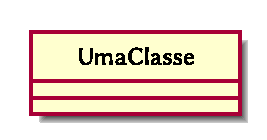
\includegraphics[scale=1]{./uml_diagrams/class0}
\end{center}
\end{columns}
\vspace{0.25cm}
\item Notar que o nome da classe inicia com maiúscula e, depois, CamelCase
\item Esta classe não pode ser executada diretamente porque não tem o método \mintinline{java}{main}
\end{itemize}
\end{frame}    
    
    
\begin{frame}[fragile]{\mintinline{java}{main()}}
    \begin{itemize}
        \item Para ser possível executar um programa Java, uma das classes do programa tem de ter o método \mintinline{java}{main}
        \item Quando mandamos correr o programa, a JVM vai à procura do \mintinline{java}{main} dentro classe que tiver o mesmo nome que ficheiro \text{.java} que estamos a correr
        \item O \mintinline{java}{main} tem uma sintaxe especial que a JVM espera:
\begin{minted}{java}
    public static void main(String[] args) {
    }
\end{minted}
    \end{itemize}
\begin{itemize}
\item \mintinline{java}{public}: permite à JVM aceder ao \mintinline{java}{main}
\item \mintinline{java}{static}: para a JVM poder executar o \mintinline{java}{main} (i.e., sem instanciar a classe)
\item \mintinline{java}{void}: para indicar que o \mintinline{java}{main} não vai retornar nenhum valor
\item \mintinline{java}{String[] args}: contém as strings passadas pelo terminal (o nome \mintinline{java}{args} é utilizado frequentemente, mas pode ser o que quisermos)
\end{itemize}
\end{frame}
    

\begin{frame}[fragile]{Programa mínimo (assumir ficheiro com nome \texttt{Treta.java})}
\begin{columns}
\column[t]{0.5\linewidth}
    \begin{minted}{java}
class Treta {
    
    public static void main(String[] args) {
        
    }
    
}
\end{minted}
\column[t]{0.5\linewidth}
\begin{center}
    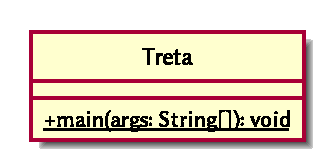
\includegraphics[width=0.5\linewidth]{./uml_diagrams/class1}
\end{center}
\end{columns}
\vfill

\begin{itemize}
    \item Notar que:
    \begin{itemize}
        \item O \mintinline{java}{main} encontra-se dentro de uma classe que tem o mesmo nome que o ficheiro
        \item Ao executarmos o programa \texttt{Treta.java}, a JVM ``vai'' à classe treta e executa o \mintinline{java}{main}
        \item Métodos estáticos aparecem sublinhados em UML
    \end{itemize}
\end{itemize}
\end{frame}


\begin{frame}[fragile]{Programa com 2 classes (ficheiro \texttt{Fichas.java})}
\begin{columns}
\column[]{0.5\linewidth}
\begin{minted}[fontsize=\small]{java}
class FichaUm {
    void exercicioUm() {
        System.out.println("Olá mundo!");
    }
    
    void exercicioDois() {
        System.out.println("Adeus mundo!");
    }
}

class Fichas {
    public static void main(String[] args) {
        FichaUm f1 = new FichaUm();
        f1.exercicioUm();
    }
}
\end{minted}
\column[]{0.5\linewidth}
\begin{center}
    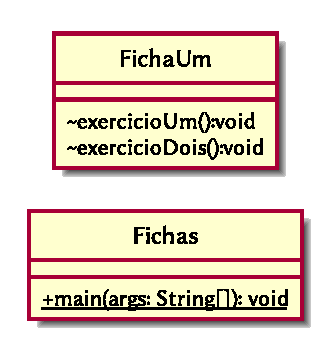
\includegraphics[width=0.5\linewidth]{./uml_diagrams/class2}
\end{center}
\vspace{0.5cm}
\tiny \textbf{NOTA:} Este é um exemplo estúpido já que, geralmente, apenas faz sentido criar uma classe se estivermos a pensar criar mais do que uma instância da mesma. Inclusivamente, o nome \texttt{Fichas} viola a convenção.
\end{columns}

\end{frame}
  
\begin{frame}[fragile]{Programa com mais sentido (ficheiro \texttt{Zoo.java})}
\begin{columns}
\column[t]{0.5\linewidth}
\begin{minted}[fontsize=\scriptsize]{java}
class Animal {
    String nome;
    
    Animal(String nome) {  // construtor
        this.nome = nome;
    }
    
    String getNome() {
        return nome;
    }
}

class Zoo {
    public static void main(String[] args) {
        Animal a1 = new Animal("Bobby");
        Animal a2 = new Animal("Pitucha");
        System.out.println("Um dos animais chama-se ", a1.nome);
    }
}
\end{minted}
\column[t]{0.5\linewidth}
\begin{itemize}
    \item 2 classes e 2 objetos:
\end{itemize}
    \begin{center}
        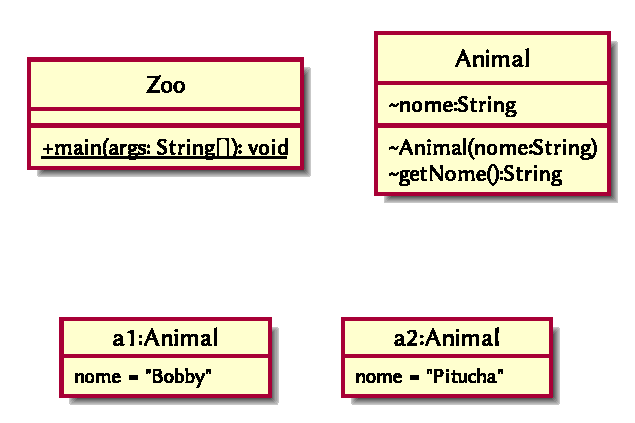
\includegraphics[width=0.6\linewidth]{./uml_diagrams/class3}
    \end{center}
\textbf{\color{red}PERIGO!} No \mintinline{java}{main}, estamos a aceder diretamente ao atributo \texttt{nome}!
\end{columns}
\vspace{-0.2cm}
\begin{flushright}
\tiny    \textbf{NOTA:} Em UML 1.0 sublinhava-se o nome e tipo dos objetos (i.e., das instâncias)
\end{flushright}
\end{frame}  

\begin{frame}[fragile]{Programa com \textit{ainda} mais sentido (ficheiro \texttt{Zoo.java})}
\begin{columns}
\column[t]{0.5\linewidth}
\begin{minted}[fontsize=\scriptsize]{java}
class Animal {
    private String nome;
    
    public Animal(String nome) {  // construtor
        this.nome = nome;
    }
    
    public String getNome() {
        return nome;
    }
}

class Zoo {
    public static void main(String[] args) {
        Animal a1 = new Animal("Bobby");
        Animal a2 = new Animal("Pitucha");
        System.out.println("Um dos animais chama-se ", a1.getNome());
    }
}
\end{minted}
\column[t]{0.5\linewidth}
\begin{center}
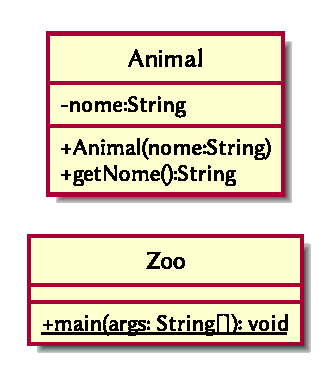
\includegraphics[width=0.4\linewidth]{./uml_diagrams/class4}
\end{center}
\begin{itemize}
    \item \mintinline{java}{a1.nome} agora não é permitido!
    \item Notar privado (--) \textit{vs} público (+)
\end{itemize}
\end{columns}
\end{frame}  


\begin{frame}[fragile]{Se o nome do animal não é conhecido à partida (ficheiro \texttt{Zoo.java})}
\begin{columns}
\column[t]{0.5\linewidth}
\begin{minted}[fontsize=\scriptsize]{java}
class Animal {
    private String nome;
    
    public String getNome() {
        return nome;
    }

    public void setNome(String nome) {
        this.nome = nome;
    }
}

class Zoo {
    public static void main(String[] args) {
        Animal a1 = new Animal();
        a1.setNome("Bobby");
        System.out.println("O bicho chama-se ", a1.getNome());
    }
}
\end{minted}
\column[t]{0.5\linewidth}
\begin{center}
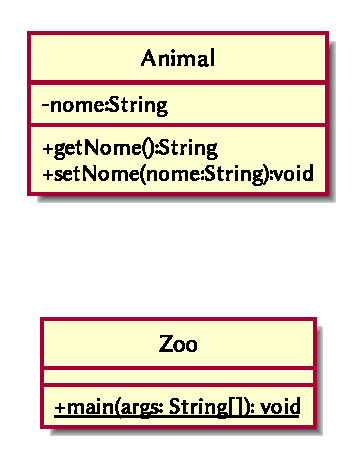
\includegraphics[width=0.45\linewidth]{./uml_diagrams/class5}
\end{center}

\end{columns}
\end{frame}  


\begin{frame}{Atributos (i.e., \textit{variáveis}) e métodos de instância \textit{vs} classe}
\begin{columns}
\column[]{0.7\linewidth}
\begin{itemize}
    \item Um atributo de instância:
    \begin{itemize}
        \item é uma \textit{variável} exclusiva de cada objeto (i.e., cada instância tem a sua própria cópia)
        \item só existe se a instância tiver sido criada
        \item se for público, acede-se através do objeto, e.g., \mintinline{java}{a1.nome}
    \end{itemize}
    \item Um atributo de classe (i.e., \mintinline{java}{static}):
    \begin{itemize}
        \item é uma \textit{variável} comum a todos os objectos instanciados a partir dessa classe
        \item acede-se, geralmente, através do nome da classe, e.g., \mintinline{java}{JFrame.ABORT}
        \item não requer a existência de um objeto dessa classe
        \item define, frequentemente, uma constante dessa classe (como no exemplo anterior)
    \end{itemize}
    \item Os métodos de instância e de classe são acedidos da mesma forma que os atributos
\end{itemize}
\column[]{0.3\linewidth}
\begin{center}
    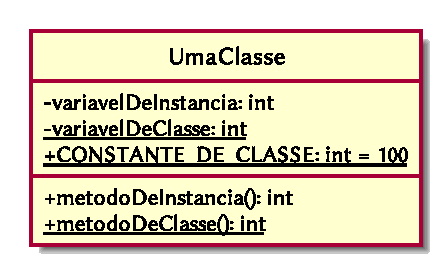
\includegraphics[width=\linewidth]{./uml_diagrams/class6}
\end{center}
\end{columns}
\end{frame}  


\section{Tipos e operadores}
\begin{frame}{Literais numéricos \textit{vs} Tipos numéricos (mais comuns)}
\begin{itemize}
    \item \mintinline{java}{int}: não tem parte decimal
    
    \hspace{0.25cm}
    \texttt{-5, 4, 8, 2000}
    \item \mintinline{java}{float}: tem parte decimal (basta sufixar com um \texttt{f})
    
    \hspace{0.25cm}
    \texttt{-5f, 4f, 8.0f, 2000.5f}
    \item \mintinline{java}{double}: tem parte decimal e mais precisão que \mintinline{java}{float}
    
    \hspace{0.25cm}
    \texttt{-5.0, 4.0, 8.0, 2000.5}
\end{itemize}
\end{frame}

\begin{frame}{Operações entre diferentes tipos}
\begin{itemize}
    \item O valor final de uma operação é do tipo mais geral
    \item Exemplo (com operador +, mas pode ser outro operador aritmético): 
    \begin{itemize}
        \item \mintinline{java}{int + float} $\rightarrow$ \mintinline{java}{float}
        \item \mintinline{java}{int + double} $\rightarrow$ \mintinline{java}{double}
        \item \mintinline{java}{float + double} $\rightarrow$ \mintinline{java}{double}
    \end{itemize}
\end{itemize}
\end{frame}

\begin{frame}[fragile]{Atribuição de valores}
\begin{itemize}
\item Para se atribuir um valor a uma variável, a variável tem de ter capacidade para receber o valor atribuído
\item Exemplos OK:
\begin{minted}{java}
    double n = 2.5;  // double cabe num double
    double n = 2.5f; // float cabe num double
    double n = 2;    // int cabe num double
    float n = 2.5f;  // float cabe num float
    float n = 2;     // int cabe num float
    int n = 2;       // int cabe num int
\end{minted}
\item Quando os tipos não são iguais, ocorre um \textbf{cast implícito} (i.e., uma conversão de tipo)
\end{itemize}
\end{frame}

\begin{frame}[fragile]{Atribuição de valores: Not OK}
\begin{itemize}
\item Exemplos que vão dar erro:
\begin{minted}{java}
    int n = 2.5;     // double não cabe num int
    int n = 2.5f;    // float não cabe num int
    float n = 2.5;   // double não cabe num float
\end{minted}
\item Para ``forçar'' a atribuição tem de se fazer um \textbf{cast explícito} para o tipo da variável recetora (o mesmo que dizer ``\textit{trust me I know what I'm doing}'')
\begin{minted}{java}
    int n = (int)2.5;     // double não cabe num int
    int n = (int)2.5f;    // float não cabe num int
    float n = (float)2.5; // double não cabe num float
\end{minted}
\item Se o valor a atribuir não ``encaixar'' na variável recetora:
\begin{itemize}
\item \mintinline{java}{int}, a parte da informação que não encaixa é descartada, por exemplo:
\begin{minted}{java}
    int n = (int)2.5;     // n contém apenas o valor 2!!!
\end{minted}
\item \mintinline{java}{float}, a variável toma o valor \mintinline{java}{Infinity}
\end{itemize} 

\item A operação de cast tem precedência sobre as operações aritméticas 
\end{itemize}
\end{frame}

\begin{frame}[fragile]{Operadores de divisão}
\begin{itemize}
    \item A divisão é efetuada pelo operador \texttt{/}
    \begin{alertblock}{Cuidado!}
        \begin{itemize}
        \item Referido anteriormente: operações aritméticas entre dois tipos, resultam no tipo mais geral
        \item Assim, se ambos operandos forem \mintinline{java}{int}, o resultado será \mintinline{java}{int}
    \begin{minted}{java}
        5/2    // O resultado é 2 em vez de 2.5
        1/2    // O resultado é 0 em vez de 0.5
    \end{minted}
    \item A solução passa por converter um dos operandos:
    \begin{minted}{java}
        1f/2    // O resultado é 0.5f
        1/2.0   // O resultado é 0.5  (i.e. double)
    \end{minted}
    \end{itemize}
    \end{alertblock}
    \item O resto da divisão é dado pelo operador \texttt{\%}
    \begin{itemize}
        \item Em Java (ao contrário do C), pode-se operar não inteiros
    \end{itemize}
\end{itemize}
\end{frame}


\begin{frame}[fragile]{Limites dos tipos primitivos}
\begin{itemize}
    \item Quantas ``caixas de memória'' são necessárias para representar o resultado de $\frac{1}{3}$?
    \item Temos de decidir: valores máximos, mínimos, e precisão que queremos representar
    \item Decidir, quer dizer: ``escolher que tipo vamos usar, \mintinline{java}{int}, \mintinline{java}{float}, etc.''
    \item Se o resultado de uma operação com \textit{não inteiros} não ``couber'' no tipo que estamos a utilizar, o resultado será \mintinline{java}{Infinity} (e.g., cast de um \mintinline{java}{double} muito grande para \mintinline{java}{float})
    \item No caso dos inteiros, temos um overflow (não é fácil de detetar)
    \item As \textit{wrapper classes} permitem consultar os valores máximos (e/ou mínimos) possíveis:
\begin{minted}{java}
Integer.MAX_VALUE // maior inteiro possível (o mais negativo é MIN_VALUE)
Float.MAX_VALUE   // maior float possível (o mais negativo é -MAX_VALUE)
Double.MAX_VALUE  // como no float
Float.MIN_VALUE   // o valor mais pequeno que é possível representar
Double.MAX_VALUE  // como no float
\end{minted}
\end{itemize}
\end{frame}


\begin{frame}{Resultados estranhos? (tipos com vírgula flutuante)}
\begin{center}
    \begin{tabular}{ccl}
\textbf{Operação} & \textbf{Resultado} & \textbf{Comentário}\\
\hline
$\frac{n}{\pm \mintinline{java}{Infinity}}$ & 0 & Algo dividido infinitamente, tende para 0\\
$\mintinline{java}{Infinity}  + \mintinline{java}{Infinity}$  &  \mintinline{java}{Infinity} & \\
$\pm \mintinline{java}{Infinity} \times \pm \mintinline{java}{Infinity}$ & $\pm \mintinline{java}{Infinity}$\\
$\frac{\pm n}{0}, \quad n \neq 0$        &   $\pm \mintinline{java}{Infinity}$ & \scriptsize Se $n$ e 0 forem \mintinline{java}{int}, temos uma \mintinline{java}{ArithmeticException}\\
$\frac{\pm 0}{\pm 0}$      &  \mintinline{java}{NaN}\\
$\pm \mintinline{java}{Infinity} - \mintinline{java}{Infinity}$ &   \mintinline{java}{NaN}\\
$\frac{\pm \mintinline{java}{Infinity}}{\pm \mintinline{java}{Infinity}}$  & \mintinline{java}{NaN}\\
$\pm \mintinline{java}{Infinity} \times 0$      &  \mintinline{java}{NaN}\\
\end{tabular}
\end{center}
\begin{block}{Decorar?}
\begin{itemize}
    \item Muito mais importante que decorar cada situação é saber que \mintinline{java}{Infinity} e \mintinline{java}{NaN} podem advir duma destas operações
\end{itemize}
\end{block}
\end{frame}

\section{Formatação de output}

\begin{frame}[fragile]{Formatar números com \mintinline{java}{DecimalFormat}}
\begin{itemize}
    \item Para valores numéricos, podemos criar um formatador
\end{itemize}
\vspace{0.5cm}
\begin{minted}{java}
    double altura = 1.785;
    String padrao = "##.##";  // ou "00.00", aparece 0 se não existir dígito
    DecimalFormat df = new DecimalFormat(padrao);
    System.out.println("A altura é " + df.format(altura));
\end{minted}
\vfill

\begin{center}
    \href{https://docs.oracle.com/javase/tutorial/i18n/format/decimalFormat.html#numberpattern}{Detalhe sobre a sintaxe dos padrões}
\end{center}
\end{frame}


\begin{frame}[fragile]{Output formatado}
\begin{itemize}
    \item Em vez de se criar uma string a partir de concatenação:
\begin{minted}{java}
int idade = 25; double alt = 1.785;
System.out.print("Idade é " + idade + ", e altura é " +  altura + "cm");
\end{minted}
\item é possível indicar onde, na string, devem aparecer os valores:
\begin{minted}{java}
System.out.format("A idade é %d, e a altura %f cm", idade, altura);
\end{minted}
        
\item O \texttt{\%d} e \texttt{\%f}, são chamados conversores para inteiros (i.e.\ decimal integers) e não inteiros (i.e.\ floating point), respetivamente

\item O formatador \texttt{\%f} permite controlar o número de casas decimais do número, e.g.\ 2 casas:
\begin{minted}{java}
System.out.format("A a altura é %.2f cm", altura);
\end{minted}

\item \mintinline{java}{System.out.format()} é equivalente a \mintinline{java}{System.out.printf()}
\end{itemize}
\end{frame}


\begin{frame}[fragile]{Alinhamento de Strings (com conversor {\color{red}\%s})}
\begin{itemize}
    \item Pode definir-se o espaço mínimo e máximo de carateres que uma String deve ocupar, bem como o seu alinhamento nesse espaço
    \item Espaço exato, texto alinhado à direita (o que acontece por omissão nas Strings):
    \begin{minted}{java}
    System.out.format("%s", "Olá")  // ou System.out.println("Olá")
    \end{minted}
    Ouput: \fbox{Olá}
    \item Espaço mínimo 10 carateres, texto alinhado à direita:
    \begin{minted}{java}
    System.out.format("%10s", "Olá");
    \end{minted}
    Ouput: \fbox{\ \ \ \ \ \ \ Olá}
    \item Espaço mínimo 10 carateres, texto alinhado à esquerda:
    \begin{minted}{java}
        System.out.format("%-10s", "Olá");
    \end{minted}
    Ouput: \fbox{Olá\ \ \ \ \ \ \ }
\end{itemize}
\end{frame}



\section{Classes e métodos úteis}
\begin{frame}[fragile]{\mintinline{java}{String}: Métodos úteis}
\begin{itemize}
\item \mintinline{java}{int length()}: Devolve o tamanho da string
\begin{minted}{java}
    String nome = "Manuel";
    System.out.println(nome.lenght());          // imprime 6
    System.out.println("Maria".length());       // imprime 5
\end{minted}
\item \mintinline{java}{char charAt(pos)}: Devolve o carater na posição \mintinline{java}{pos}
\begin{minted}{java}
    System.out.println(nome.charAt(2));        // imprime 'n'
\end{minted}

\item \mintinline{java}{String substring(posI, posF)}: Devolve a sub-string de \mintinline{java}{posI} até \mintinline{java}{posF} (não inc.)
\begin{minted}{java}
    int pos = 5;
    System.out.println(nome.substring(2, pos));  // imprime "nue"
\end{minted}

\item \mintinline{java}{String concat(String)}: Concatena as duas strings
\begin{minted}{java}
    System.out.println("Olá".concat(" Maria"));  // "Olá Maria"
\end{minted}

\item \mintinline{java}{public int indexOf(char)}: Devolve posição do caráter (um \mintinline{java}{int} na realidade)
\begin{minted}{java}
    System.out.println("Olá".indexOf('o'));  // imprime 1
\end{minted}
\end{itemize}
\end{frame}

\begin{frame}[fragile]{\mintinline{java}{concat} vs \mintinline{java}{+}}
\begin{itemize}
    \item O código
    \begin{minted}{java}
    System.out.println("Olá".concat(" Maria"));  // "Olá Maria"
    \end{minted}
é parecido com:

  \begin{minted}{java}
    System.out.println("Olá" + " Maria");  // "Olá Maria"
\end{minted}

    \item Isto quer dizer que, ao se utilizar o \mintinline{java}{+}, um dos operandos \textbf{tem de ser} uma \mintinline{java}{String}, para que o resultado seja uma \mintinline{java}{String}
    \item Situações problemáticas:
\begin{minted}{java}
System.out.println('A' + 'b'); // Adição de chars resulta em int!
System.out.println("Olá".charAt(1) + "bom".charAt(0) + "dia");
\end{minted}
\begin{itemize}
    \item No último exemplo, somamos 2 \mintinline{java}{char}s que resultam num \mintinline{java}{int} e, depois, esse número concatena com a \mintinline{java}{String} ``dia''
    \item Relembrar que \mintinline{java}{charAt} devolve um \mintinline{java}{char} e não uma \mintinline{java}{String}
\end{itemize}

\end{itemize}
\end{frame}


\begin{frame}[fragile]{\mintinline{java}{Math}: Métodos úteis}
\begin{itemize}
\item \mintinline{java}{static double pow(double a, double b)}: Devolve $a^b$
\begin{minted}{java}
    System.out.println(Math.pow(2, 3));  // imprime 8
\end{minted}
\item \mintinline{java}{static double floor(double a)}: Devolve $a$ arredondado para baixo
\begin{minted}{java}
    System.out.println(Math.floor(2.9));  // imprime 2
\end{minted}
\item \mintinline{java}{static double ceil(double a)}: Devolve $a$ arredondado para cima
\begin{minted}{java}
    System.out.println(Math.ceil(2.1));  // imprime 3
\end{minted}
\item \mintinline{java}{static int round(float a)}: Devolve $a$ arredondado ao inteiro mais próximo
\begin{minted}{java}
    System.out.println(Math.round(2.1));  // imprime 2
\end{minted}
\end{itemize}
\vfill

\begin{alertblock}{Atenção!}
\begin{itemize}
    \item Notar que os métodos (e atributos) da classe \mintinline{java}{Math} são todos \textbf{static}, i.e., de classe
    \item Assim nunca instanciamos a classe \mintinline{java}{Math} (i.e., nunca se criam objetos desta classe)
    \item Todos os membros da classe são acedidos através nome da classe, e não através do objeto
\end{itemize}
\end{alertblock}
\end{frame}

\begin{frame}[fragile]{\mintinline{java}{Scanner}: Métodos úteis}
\begin{itemize}
    \item \mintinline{java}{String next()}: Lê até ao próximo espaço e devolve uma string
\begin{minted}{java}
    Scanner sc = new Scanner(System.in);
    String frase = sc.next();      // Digitar: "Olá bom dia"
    System.out.println(frase);     // imprime "Olá"
\end{minted}

\item \mintinline{java}{String nextLine()}: Lê até ao próximo enter e devolve uma string
\begin{minted}{java}
    String frase = sc.nextLine();  // Digitar: "Olá bom dia"
    System.out.println(frase);     // imprime "Olá bom dia"
\end{minted}

\item \mintinline{java}{String nextInt()}: Lê e devolve um número inteiro
\begin{minted}{java}
    int valor = sc.nextInt();
\end{minted}
\item \mintinline{java}{float nextFloat()}: Lê e devolve um número \textit{floating point} (vírgula flutuante)
\begin{minted}{java}
    float valor = sc.nextFloat();
\end{minted}
\item \mintinline{java}{double nextDouble()}: Lê e devolve um número \textit{floating point} de precisão dupla
\begin{minted}{java}
    double valor = sc.nextDouble();
\end{minted}
\item \mintinline{java}{void close()}: Fecha o scanner (nunca fechar antes de ler tudo o que queremos!!!)
\begin{minted}{java}
    sc.close();
\end{minted}
\end{itemize}
\end{frame}

\begin{frame}[fragile]{Ler do teclado}
\begin{itemize}
    \item A forma mais fácil de ler valores introduzidos através do teclado é utilizando um objeto da classe \mintinline{java}{Scanner} (temos de importar do package \mintinline{java}{java.util})
    \item Os objetos da classe \mintinline{java}{Scanner} precisam de saber onde queremos fazer o \textit{scan}
    \item Em Java, ``teclado'' diz-se: \mintinline{java}{System.in}
    \item Portanto, podemos ler do teclado assim:
\begin{minted}{java}
 Scanner sc = new Scanner(System.in);  // instância p/ler no teclado
 String nome = sc.next();
 String morada = sc.nextLine();
 int idade = sc.nextInt();
 float altura = sc.nextFloat();  // ou double altura = sc.nextDouble()
 sc.close();  // fechar quando não for necessário ler mais nada
\end{minted}
\end{itemize}
\end{frame}

\begin{frame}[fragile]{Escrever no ecrã}
\begin{itemize}
    \item Em Java, ``ecrã'' diz-se: \mintinline{java}{System.out}\footnote{\mintinline{java}{out} é, um atributo da classe \mintinline{java}{System}, instância da classe \mintinline{java}{PrintStream} e que a JVM `canaliza' para o ecrã} 
    \item Podemos escrever no ecrã por enviar a mensagem \mintinline{java}{print} ao ``ecrã''
\begin{minted}{java}
    System.out.print("Olá");
\end{minted}
\item O ``ecrã'' sabe responder a outras mensages, p.ex., \mintinline{java}{println} que, além de imprimir a mensagem desejada, também muda de linha
\item São equivalentes:
\begin{minted}{java}
    System.out.println("Olá");
    System.out.print("Olá\n");
\end{minted}
\mintinline{java}{'\n'} é um caráter invisível que representa uma nova linha (new line)
\end{itemize}
\end{frame}


\begin{frame}[fragile]{Importar?}
\begin{itemize}
\item Porque é que temos acesso às classes \mintinline{java}{String} e \mintinline{java}{Math} sem ter de importar?
\begin{itemize}
    \item Estão ambas no package \mintinline{java}{java.lang} que é importado automaticamente pela JVM
\end{itemize}
\item As classes no package \mintinline{java}{java.util} não são importadas automaticamente
\begin{itemize}
    \item Por isso é que, para utilizar a classe \mintinline{java}{Scanner}, precisamos de importar:
    \begin{minted}{java}
    import java.util.Scanner;
    \end{minted}
\end{itemize}
\end{itemize}
\end{frame}

\section{Controlo de acesso aos membros}
\begin{frame}{Controlo de acesso aos membros da classe}
\begin{itemize}
    \item Os membros de uma classe são os:
    \begin{itemize}
        \item Atributos (i.e., as variáveis disponíveis na classe)
        \item Métodos (i.e., as ``funções'' definidas na classe)
    \end{itemize}
    \item Podemos controlar o acesso aos membros usando as palavras chave:
    \begin{itemize}
        \item \mintinline{java}{private} (\textbf{--} em UML): Ninguém fora da classe pode aceder
        \item \mintinline{java}{public}  (\textbf{+} em UML): Todos fora da classe podem aceder
        \item Há mais 2, mas ficam para mais tarde
    \end{itemize}
\end{itemize}
\vfill

\begin{block}{Qual usar?}
\begin{itemize}
    \item Regra geral (para simplicar):
    \begin{itemize}
        \item Atributos devem ser privados
        \item Métodos devem ser públicos
    \end{itemize}
    \item Dito isto, há atributos que faz sentido serem públicos e métodos que faz sentido serem privados (quando tiverem mais experiência)
\end{itemize}
\end{block}
\end{frame}


\begin{frame}[fragile]{\mintinline{java}{public} \textit{vs} \mintinline{java}{private}}
\begin{columns}
\column[]{0.5\linewidth}
\begin{minted}[fontsize=\scriptsize]{java}
class Animal {
    public String especie;
    
    public String getEspecie(){
        return especie;
    }

    public void setEspecie(String e) {
        especie = e;
    }
}

class Treta {
    public static void main(String[] args) {
        Animal a = new Animal();
        a.especie = "Carapau";              // OK
        a.setEspecie("Galinha");            // OK
        System.out.println(a.getEspecie()); // OK
    }
}
\end{minted}

\column[]{0.5\linewidth}
\begin{minted}[fontsize=\scriptsize]{java}
class Animal {
    private String especie;
    
    private String getEspecie(){
        return especie;
    }
    
    public void setEspecie(String e) {
        especie = e;
    }
}

class Treta {
    public static void main(String[] args) {
        Animal a = new Animal();
        a.especie = "Carapau";     // NÃO OK !!!
        a.setEspecie("Galinha");   // OK
        System.out.println(a.getEspecie());//NÃO OK!
    }
}
\end{minted}
\end{columns}
\end{frame}


\begin{frame}[fragile]{Controlo de acesso a classes}
\begin{itemize}
    \item É possível controlar o acesso à classe por parte de código noutras classes e packages
    \item Este é conteúdo para mais tarde, mas fica aqui um aviso muito importante:
    \begin{alertblock}{AVISO!!!}
        \begin{itemize}
            \item Alguns dos exercícios no Moodle podem requerer que a classe onde está o \mintinline{java}{main} seja pública
        \end{itemize}
    \end{alertblock}
\end{itemize}
\begin{columns}
\column[]{0.5\linewidth}
\begin{itemize}
\item Se isto não funcionar:
\begin{minted}{java}
class Treta {  // sem public
    public static void main(){
        System.out.println("Olá");
    }
}
\end{minted}
\end{itemize}
\column[]{0.5\linewidth}
\begin{itemize}
    \item Experimentar isto:
\begin{minted}{java}
public class Treta {  // com public
    public static void main(){
        System.out.println("Olá");
    }
}
\end{minted}
\end{itemize}
\end{columns}
\end{frame}

\section{Operadores lógicos, relacionais, e decidir}
\begin{frame}{Tipo de dados \mintinline{java}{boolean}}
\begin{itemize}
    \item Apenas 2 valores possíveis (ou \mintinline{java}{null} se não for inicializado):
    \begin{itemize}
        \item Verdadeiro: \mintinline{java}{true}
        \item false: \mintinline{java}{false} 
    \end{itemize}
\item São chamados de valores lógicos
\item Existem operadores para operar estes valores
\end{itemize}
\end{frame}


\begin{frame}[fragile]{Operadores lógicos}
\begin{itemize}
    \item \textbf{And} lógico: \mintinline{java}{&&}
    \begin{itemize}
        \item Resulta em \mintinline{java}{true} se \textbf{ambos} operadores forem \mintinline{java}{true}, ou \mintinline{java}{falso} caso contrário
    \end{itemize}
    \begin{minted}{java}
    System.out.print(true && true);  // imprime true
    System.out.print(true && false); // (ou false && true) imprime false
    \end{minted}
    \item \textbf{Or} lógico: \mintinline{java}{||}
    \begin{itemize}
        \item Resulta em \mintinline{java}{true} se \textbf{um} dos operandos for \mintinline{java}{true}, ou \mintinline{java}{false} caso contrário
    \end{itemize}
    \begin{minted}{java}
    System.out.print(true || true);  // imprime true
                                     // ou true||false; ou false||true 
    System.out.print(false || false);// false (apenas se ambos false)
    \end{minted}
    \item \textbf{Not} lógico: \mintinline{java}{!}
    \begin{itemize}
        \item Operador unário que nega o valor lógico
    \end{itemize}
    \begin{minted}{java}
    System.out.print(!true);   // imprime false
    System.out.print(!false);  // imprime true
    \end{minted}
    \end{itemize}
\end{frame}


\begin{frame}[t]{Operadores lógicos: Resumo}
\begin{center}
        \begin{columns}
        \column[]{0.33\linewidth}
        \begin{tabular}{cc}
            \textbf{Operação} & \textbf{Res}\\
            \hline
            \mintinline{java}{false && false} & \mintinline{java}{false}\\
            \mintinline{java}{false && true} & \mintinline{java}{false}\\
            \mintinline{java}{true && false} & \mintinline{java}{false}\\
            \mintinline{java}{true && true} & \mintinline{java}{true}\\
        \end{tabular}
        
        \column[]{0.33\linewidth}
        \begin{tabular}{cc}
            \textbf{Operação} & \textbf{Res}\\
            \hline
            \mintinline{java}{false || false} & \mintinline{java}{false}\\
            \mintinline{java}{false || true} & \mintinline{java}{true}\\
            \mintinline{java}{true || false} & \mintinline{java}{true}\\
            \mintinline{java}{true || true} & \mintinline{java}{true}\\
        \end{tabular}
        
        \column[]{0.33\linewidth}
        \begin{tabular}{cc}
            \textbf{Operação} & \textbf{Res}\\
            \hline
            \mintinline{java}{!false} & \mintinline{java}{true}\\
            \mintinline{java}{!true} & \mintinline{java}{false}\\
        \end{tabular}
    \end{columns}
\end{center}
    \vfill
    \begin{itemize}
        \item Precedências: 
        \begin{itemize}
            \item $1^\text{st}$ \mintinline{java}{!}; $2^\text{nd}$ \mintinline{java}{&&}; $3^\text{rd}$ \mintinline{java}{||}
            \item Pensem no negativo (menos unário), multiplicação e adição
            \item Pode alterar-se com a utilização de parêntesis
        \end{itemize}
        \item Operadores lógicos têm precedência inferior à dos operadores relationais (a seguir)
    \end{itemize}
    
\end{frame}



\begin{frame}[fragile]{Operadores relacionais}
\begin{itemize}
\item Não é frequente escrever-se \mintinline{java}{true} ou \mintinline{java}{false} diretamente em expressões
\item Valores booleanos resultam, frequentemente, de operações relacionais (i.e., comparações)
\item Um operador relacional estabelece a relação entre 2 valores
\item Por exemplo: ``10 é menor que 20?''
\begin{minted}{java}
    System.out.print(10 < 20);  // imprime: true
\end{minted}
\end{itemize}
\end{frame}


\begin{frame}{Operadores relacionais: Resumo}
    \begin{center}
        \begin{tabular}{clrr}
            \rowcolor[HTML]{000000} 
            {\color[HTML]{EFEFEF} \textbf{Operador}} & \multicolumn{1}{c}{\cellcolor[HTML]{000000}{\color[HTML]{EFEFEF} \textbf{Operação}}} & \multicolumn{1}{c}{\cellcolor[HTML]{000000}{\color[HTML]{EFEFEF} \textbf{Exemplo 1}}} & \multicolumn{1}{c}{\cellcolor[HTML]{000000}{\color[HTML]{EFEFEF} \textbf{Exemplo 2}}} \\
            \textless{}                            & Menor que                                                                             & 10 \textless\ 20 → true                                                                & 20 \textless\ 10 → false                                                               \\
            \rowcolor[HTML]{C0C0C0} 
            \textgreater{}                         & Maior que                                                                          & 5 \textgreater\ 2 → true                                                               & 2 \textgreater\ 5 → false                                                              \\
            \textless{}=                           & Menor ou igual que                                                                 & 8 \textless{}= 10 → true                                                              & 8 \textless{}= 8 → true                                                               \\
            \rowcolor[HTML]{C0C0C0} 
            \textgreater{}=                        & Maior ou igual que                                                              & 4 \textgreater{}= 1 → true                                                            & 4 \textgreater{}= 4 → true                                                            \\
            ==                                     & Igual a                                                                              & 6 == 6 → true                                                                         & 3 == 6 → false                                                                        \\
            \rowcolor[HTML]{C0C0C0} 
            !=                                     & Não igual a (diferente)                                                              & 2 != 7 → true                                                                         & 8 != 8 → false                                                                       
        \end{tabular}
    \end{center}
    \vfill
    \begin{itemize}
        \item Operadores relacionais têm precedência mais elevada que os lógicos
        \item Pensar nos operadores relacionais como uma pergunta à qual a resposta apenas pode ser \mintinline{java}{true} ou \mintinline{java}{false}
    \end{itemize}
\end{frame}


\begin{frame}[fragile]{Executar ou não executar}
\begin{itemize}
    \item Dependendo do resultado de uma operação relacional, podemos decidir se queremos, ou não executar uma (ou mais) instrução
    \item A instrução \mintinline{java}{if} é uma das que permite fazer isso
    \item Sintaxe:
\begin{minted}{java}
    if (valorLógico)
        instruçãoAExecutar; 
\end{minted}
a instrução só será executada se o valor lógico for \mintinline{java}{true}
\item Recordar que os valores lógicos resultam de operações relacionais (i.e., comparações)
\item Se tivermos mais do que uma instrução a executar, utilizamos chavetas:
    \begin{minted}{java}
    if (valorLógico) {
        instrução1;
        instrução2;
    }
\end{minted}
\end{itemize}
\end{frame}


\begin{frame}[fragile]{Executar de entre duas alternativas}
\begin{itemize}
    \item É possível executar alternativas dependendo do valor lógico
    \begin{minted}{java}
     if (valorLógico)
        instruçãoAExecutar;   // executa se valorLógico for true
     else
        instruçãoAlternativa; // executa se nenhum dos valores 
                              // lógicos anteriores for true
    \end{minted}
\item Notar que se uma das instruções (ou bloco de instruções) for executada, mais nenhuma no \mintinline{java}{if} será
\item Aplica-se a mesma regra da utilização de chavetas para executar grupos de instruções
\end{itemize}
\end{frame}


\begin{frame}[fragile]{Executar de entre \textbf{mais de duas} alternativas}
\begin{itemize}
\item É possível executar várias alternativas dependendo de vários valores lógicos
\begin{minted}{java}
    if (valorLógico1)
        instruçãoAExecutar;    // executa se valorLógico for true
    else if (valorLógico2)
        instruçãoAlternativa1;
    else
        instruçãoAlternativa2; // executa se nenhum dos valores 
                               // lógicos anteriores for true
\end{minted}
\item Podemos ter quantos \mintinline{java}{else if} desejarmos
\item Notar que sempre que aparece \mintinline{java}{if}, tem de haver um valor lógico (i.e., condição)
\item O \mintinline{java}{else} isolado apenas pode aparecer no fim (como alternativa final)
\item Aplica-se a mesma regra da utilização de chavetas para executar grupos de instruções
\end{itemize}
\end{frame}


\begin{frame}[fragile]{Muitas comparações com a mesma variável \mintinline{java}{int} (\mintinline{java}{==})}
\begin{columns}[t]

\column[]{0.25\linewidth}
\begin{minted}[fontsize=\footnotesize]{java}
    if (a == 5) {
        s = 50;
        a = 0;
    } else if (a == 10) {
        s = 2;
        a = 5;
    } else if (a == 20) {
        s = 30;
        a = 200;
    } else {
        s = 34;
        a = 15;
    }
\end{minted}
\column[]{0.5\linewidth}
\begin{itemize}
    \item \mintinline{java}{if} é complicado de ler se tivermos de ver se uma variável é um de muitos valores inteiros (ou strings)
    \item Nesta situação recomenda-se a utilização da instrução \mintinline{java}{switch}
    \item Notar que o \mintinline{java}{default} funciona como o \mintinline{java}{else} final, e também é opcional
    \item O \mintinline{java}{break} impede que, depois de executar o código, a comparação continue e outro código no \mintinline{java}{switch} seja executado
\end{itemize}
\column[]{0.25\linewidth}
\begin{minted}[fontsize=\footnotesize]{java}
switch (a) {
    case 5:
        s = 50;
        a = 0;
        break;
    case 10:
        s = 2;
        a = 5;
        break;
    case 20:
        s = 30;
        a = 200;
        break;
    default:
        s = 34;
        a = 15;
}
\end{minted}
\end{columns}
\end{frame}

\begin{frame}[fragile]{Impressionar os/as amigos/amigas}



\begin{minted}{java}
        int a = 10;
        
        if (a == 10) {
            System.out.print("Dez");
        } else {
            System.out.print("Outro");
        }
\end{minted}
\begin{itemize}
    \item O \mintinline{java}{if}$\ldots$\mintinline{java}{else} pode ser substituído pelo operador ternário condicional
\end{itemize}
\begin{minted}{java}
        System.out.print(a==10 ? "Dez" : "Outro");
\end{minted}

\end{frame}

\section{Ciclos}

\begin{frame}[fragile]{\mintinline{python}{while}}
\begin{itemize}
    \item Quando não sabemos à partida o número de vezes que queremos repetir a instrução (ou bloco de instruções)
    \item Sintaxe:
    \begin{minted}{java}
    while (condição) {
        instrução1;
        instrução2;
    }
    \end{minted}
    \item As instruções repetem-se enquanto a \mintinline{java}{condição} for \mintinline{java}{true}
    \item Alguma das instruções dentro do ciclo, terá de alterar o resultado da \mintinline{java}{condição}, senão repete para sempre
\end{itemize}
\end{frame}


\begin{frame}[fragile]{\mintinline{java}{do} $\ldots$ \mintinline{java}{while}}
    \begin{itemize}
        \item Quando não sabemos à partida o número de vezes que queremos repetir as instruções
        \item Mas queremos que execute as instruções \textbf{pelo menos 1 vez}
        \item Sintaxe:
        \begin{minted}{java}
            do {
                instrução1;
                instrução2;
            } while (condição);
        \end{minted}
        \item As instruções repetem-se enquanto a \mintinline{java}{condição} for \mintinline{java}{true}
        \item Alguma das instruções dentro do ciclo, terá de alterar o resultado da \mintinline{java}{condição}, senão repete para sempre
        \item Esta tem um ponto-e-vírgula no fim
    \end{itemize}
\end{frame}


\begin{frame}[fragile]{\mintinline{java}{for}}
\begin{itemize}
    \item Quando sabemos à partida o número de vezes que queremos executar as instruções
    \begin{minted}{java}
    for (variável; condição; atualização) {
        instruções;
    }
    \end{minted}
\item Executa enquanto a \mintinline{java}{condição} for \mintinline{java}{true}
\item Podemos utilizar a \mintinline{java}{variável}:
\begin{itemize}
    \item para definir a condição
    \item dentro do ciclo
    \item na secção \mintinline{java}{atualização} (e.g., alterar a variável a cada passo)
\end{itemize} 

\begin{block}{Importante!}
\begin{itemize}
    \item a \mintinline{java}{variável} é `executada' antes de executar a \mintinline{java}{condição} e o bloco
    \item a \mintinline{java}{condição} é `executada' antes de executar o bloco
    \item a \mintinline{java}{atualização} é feita depois de executar o bloco
\end{itemize}
\end{block}


\end{itemize}
\end{frame}

\begin{frame}[fragile]{\mintinline{java}{for}: exemplos}
\begin{columns}
\column[]{0.5\textwidth}
\begin{minted}{java}
    for (int i=0; i < 10; i=i+1) {
        System.out.println(i);
    }
\end{minted}
\begin{minted}{java}
    for (int i=0; i < 10; i+=1) {
        System.out.println(i);
    }
\end{minted}
\begin{minted}{java}
    for (int i=0; i < 10; i++) {
        System.out.println(i);
    }
\end{minted}
\column[]{0.5\textwidth}
\begin{minted}{java}
    for (int i=0; i < 10; i=i+5) {
        System.out.println(i);
    }
\end{minted}
\begin{minted}{java}
    for (int i=0; i < 10; i+=5) {
        System.out.println(i);
    }
\end{minted}
\begin{minted}{java}
    for (int i=10; i >= 0; i--) {
        System.out.println(i);
    }
\end{minted}
\end{columns}

\end{frame}

\begin{frame}[fragile]{\mintinline{java}{for}: mais um exemplo}
\begin{itemize}
    \item Calcular o valor da seguinte série:
    $$S = 1000 + 100 + 10 + 1 + 0.1 + 0.01 + 0.001$$
\end{itemize}
\begin{onlyenv}<2>
 \begin{minted}{java}
     double s = 0.0; // obrigatório, senão s pode conter qualquer coisa <> 0
     for (double x = 1000; x >= 0.001; x /= 10) {
         s += x;
     }
     System.out.format("%.2f\n", s);
 \end{minted}
\end{onlyenv}
\end{frame}




\section{Revisões}

\begin{frame}{Revisão: Classe}
\begin{columns}
\column[]{0.6\linewidth}
\begin{itemize}
    \item Podemos ver uma classe como se fosse uma planta de uma casa
    \begin{itemize}
        \item A planta define as características das casas que serão feitas a partir desta (ninguém mora numa planta)
        \item As casas feitas a partir desta são objetos dessa planta (a coisa concreta)
    \end{itemize}
\end{itemize}
\column[]{0.4\linewidth}
\begin{center}
    
\includegraphics[width=\linewidth]{./figures/blueprint}
\end{center}
\end{columns}
\end{frame}

\begin{frame}{Revisão: Classe \textit{vs} Objeto}
\begin{columns}
\column[]{0.5\linewidth}
\begin{center}
    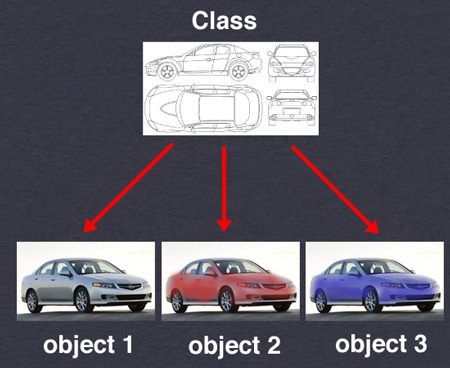
\includegraphics[width=\linewidth]{figures/car}
\end{center}
\column[]{0.5\linewidth}
\begin{itemize}
    \item \textbf{Classe} é uma espécie de desenho (i.e., planta) que define as características dos objetos que vamos produzir
    \item \textbf{Objectos} são as coisas que fazemos tendo como base o desenho (i.e., a classe)
    \item A classe define-se uma vez, e não queremos saber mais dela
    \item O que nos interessa, no fim, são os objetos (ninguém consegue viajar num desenho, tem de ter um carro concreto)
\end{itemize}
\end{columns}
\end{frame}


\begin{frame}{O que já sabemos até agora}
\begin{itemize}
    \item Uma classe pode ser vista como a definição de um tipo (serve de molde)
    \item Um objeto é um exemplo (i.e., instância) de um elemento desse \textit{tipo} (trabalhamos com os objetos)
    \item Por exemplo, \mintinline{java}{"Olá"} e \mintinline{java}{"Adeus"} são duas instâncias da classe \mintinline{java}{String}
    \item \mintinline{java}{"Olá"} tem as características definidas na classe \mintinline{java}{String}, e sabe responder às mensagens (i.e., métodos) definidas na classe \mintinline{java}{String}
    \item Para criar um objeto (i.e., instância) de uma classe, utilizamos a palavra \mintinline{java}{new} seguida do nome do tipo (i.e., classe) do objeto que queremos criar (String é um caso especial que não obriga a isso)
\end{itemize}
\end{frame}


\begin{frame}[fragile]{Exemplo}
\scriptsize
\begin{columns}
\column[t]{0.35\linewidth}
\begin{itemize}
    \item A ``planta'' (i.e., \textbf{classe}):
\begin{minted}{java}
class Animal {
    static int MAX_IDADE = 15;
    String nome;
    
    Animal(String nome) {
        this.nome = nome;
    }

    String getNome() {
        return nome;
    }

    void setNome(String nome) {
        this.nome = nome;
    }
}
\end{minted}
\end{itemize}
\column[t]{0.65\linewidth}
\begin{itemize}
\item Os \textbf{objetos}:
\begin{minted}{java}
Animal a1 = new Animal("Bobby");
Animal a2 = new Animal("Tareco");
Animal a3 = new Animal("Pituxa");
\end{minted}
\item Cada objeto é totalmente independente e:
\begin{itemize}
    \scriptsize
    \item tem o seu próprio atributo \mintinline{java}{nome}
\begin{minted}{java}
System.out.println(a1.nome);  // imprime "Bobby"
\end{minted}
\item sabe responder às mensagens \mintinline{java}{getNome} e \mintinline{java}{setNome}\begin{minted}{java}
System.out.println(a3.getNome());  // imprime "Pituxa"
\end{minted}
\end{itemize} 
porque os objetos foram criados seguindo a informação na ``planta''
\end{itemize}
\vfill

\begin{alertblock}{Importante!}
 \begin{itemize}
     \item Atributos ou métodos declarados como \mintinline{java}{static} não fazem parte do objeto
     \item São da ``planta'', e chamados a partir do nome da classe e não do objeto
     
     Por exemplo: \mintinline{java}{Animal.MAX_IDADE}  \textit{vs} \mintinline{java}{a3.nome}
 \end{itemize}
\end{alertblock}
\end{columns}
\end{frame}


\section{Sobrecarga de construtores e de métodos}

\begin{frame}[fragile]{Sobrecarga de construtores (dentro da classe, claro)}
\begin{columns}
\column[t]{0.37\linewidth}
\scriptsize
\begin{minted}{java}
 public Animal() {
    this.nome = "Bobby";
 }

 public Animal(String nome) {
    this.nome = nome;
 }

 public Animal(String especie) {
    this.especie = especie;
 }

 public Animal(int idade) {
    this.idade = idade;
 }

 public Animal(String nome, int idade) {
    this.nome = nome;
    this.idade = idade;
 }
\end{minted}

\column[t]{0.3\linewidth}
\scriptsize
\begin{itemize}
\item O que o compilador vê:
\begin{minted}{java}
public Animal(void) {
    this.nome = "Bobby";
}

public Animal(String) {
    this.nome = nome;
}

public Animal(String) {
    this.especie = especie;
}

public Animal(int) {
    this.idade = idade;
}

public Animal(String, int) {
    this.nome = nome;
    this.idade = idade;
}
\end{minted}
\end{itemize}

\column[t]{0.38\linewidth}
\scriptsize
\begin{itemize}
\item Para distinguir entre construtores, analisar:
\begin{itemize}
    \scriptsize
    \item Quantidade de parâmetros
    \item Tipo dos parâmetros
    \item Ordem dos parâmetros
\end{itemize}
\item Se os 3 critérios forem iguais, não há forma de distinguir
\item Por exemplo, não é possível distinguir entre o 2° e 3° construtores:
\begin{minted}{java}
    Animal a = new Animal("Olá");
\end{minted}
\item Qual dos 2 que recebe uma String está a ser chamado?!
\end{itemize}
\end{columns}
\end{frame}



\begin{frame}[fragile]{Sobrecarga de métodos}
\begin{columns}
\column[t]{0.55\linewidth}
\begin{itemize}
\item Vários métodos com mesmo nome
\item Mesma lógica que para os construtores: métodos com o mesmo nome são considerados diferentes se:
\begin{itemize}
\item O número de parâmetros for diferente
\item O tipo de parâmetros for diferente
\item A ordem dos (tipos dos) parâmetros for diferente
\end{itemize}
\item Nesta análise, os nomes dos parâmetros são ignorados
\item Compilador faz a mesma análise que um humano faria: Qual estou a chamar?
\begin{minted}{java}
    objeto.setInfo("Olá", 7);
\end{minted}
\end{itemize}
\column[t]{0.45\linewidth}
\begin{itemize}

\begin{minted}{java}
void setInfo(String) {
}

void setInfo(String, String) {
}

void setInfo(String, int) {
}

void setInfo(int, String) {
}
\end{minted}
\item Não há qualquer confusão entre os anteriores
\end{itemize}
\end{columns}
\end{frame}


\begin{frame}[fragile]{Construtores a chamar construtores}
\begin{columns}
\column[t]{0.5\linewidth}
\begin{itemize}
    \item Um construtor pode chamar outros construtores na mesma classe
    \item Dentro de um construtor, referimo-nos a outro construtor da classe utilizando:
    \begin{minted}{java}
        this();
    \end{minted}
    \item Dentro dos parêntesis, colocamos os argumentos requeridos pelo construtor que queremos chamar
    \item \mintinline{java}{this(...)} tem de ser a primeira coisa a acontecer no construtor
    \item O que vai acontecer?
    \begin{minted}{java}
     Animal a = new Animal();
    \end{minted}
\end{itemize}
\column[t]{0.5\linewidth}
\begin{minted}{java}
class Animal {
    String nome;
    
    Animal() {
        // não pode haver código aqui
        this("Desconhecido");
        // pode haver mais código aqui
    }
    
    Animal(String nome) {
        this.nome = nome;
    }
}
\end{minted}
\end{columns}
\end{frame}



\section{Enumerados}


\begin{frame}[fragile]{Enumerados}
\begin{itemize}
\item Um enumerado pode ser visto como um tipo de dados, que apenas pode assumir os valores definidos nele
\item Por exemplo:
\begin{minted}{java}
enum Cor {
    VERMELHO, VERDE, AZUL
}
\end{minted}
\item Os valores são escritos em maiúsculas visto que são constantes (é implícito)
\item Cada constante tem um valor inteiro que inicia em 0 (pode ser alterado)
\item Experimente imprimir as constantes
\end{itemize}

\end{frame}


\begin{frame}[fragile]{\mintinline{java}{enum}: exemplos de utilização}
    \scriptsize
\begin{columns}
\column[t]{0.5\linewidth}
\begin{itemize}
\item Normalmente:
\begin{minted}{java}
void printCor(Cor c) {
    if (c == Cor.VERMELHO)
        System.out.println("Cor vermelha");
    else if (c == Cor.VERDE)
        System.out.println("Cor verde");
    else
        System.out.println("Cor verde");
}
\end{minted}
$\vdots$

$\vdots$
\begin{minted}{java}
printCor(Cor.AZUL);
\end{minted}
\end{itemize}
\column[t]{0.5\linewidth}
\begin{itemize}
    \item Num \mintinline{java}{switch}:
\end{itemize}
\begin{minted}{java}
void printCor(Cor c) {
    switch(c) {
        VERMELHO:  // não utilizar o nome do enum
            System.out.println("Cor vermelha");
            break;
        VERDE:
            System.out.println("Cor verde");
            break;
        default:
            System.out.println("Cor azul");
    }
}
\end{minted}
\end{columns}
\end{frame}

\section{Packages}

\begin{frame}[fragile]{Package}
    \begin{itemize}
        \item De forma simples, uma pasta com ficheiros \texttt{.java} relacionados entre si
        \item Exemplo: pasta \texttt{java/util} contém os ficheiros \texttt{Scanner.java}, \texttt{ArrayList.java}, etc.
        \item Cada um desses ficheiros ``diz'' que faz parte dessa pasta por escrever
        \begin{minted}{java}
            package java.util;
        \end{minted}
        na primeira linha do código
        \item Resumindo, para criar um package\footnote{No VSCode, se estivermos num projeto, apenas temos de escolher ``New Package'', o VSCode trata de tudo.}:
        \begin{enumerate}
            \item Criar a estutura de pastas desejada
            \item Colocar os ficheiros \texttt{.java} lá dentro
            \item Escrever na primeira linha de cada ficheiro \mintinline{java}{package nomes.das.pastas}
        \end{enumerate}
        \item O ponto a separar os nomes das pastas indicam que as pastas estão dentro das outras
        \item Por exemplo, o package \mintinline{java}{java.util} corresponde à estrutura de pastas  \texttt{java/util}, i.e., a pasta \texttt{util} está dentro da pasta \texttt{java}
    \end{itemize}
\end{frame}




\begin{frame}[fragile]{Utilizar um package}
\begin{itemize}
\item Para utilizar os ``ficheiros'' que estão no package, temos de importá-los:
\begin{minted}{java}
    import nomepackage.NomeFicheiro;
\end{minted}
\item Quando fazemos \mintinline{java}{import pasta.Ficheiro}, a MV do Java precisa de saber onde está a pasta (i.e., package)
\item A MV vai procurar nas pastas que estiverem definidas numa variável de sistema chamada \texttt{CLASSPATH}
\item No terminal podemos dizer para procurar noutros sítios, utilizando o parâmetro \texttt{-cp}
\item No VSCode:
\begin{itemize}
    \item Se o package foi criado com ``New Package'', o VSCode trata de tudo
    \item Sem projeto criado, é-nos perguntado se queremos adicionar a pasta à \texttt{CLASSPATH}
    \item Poderá ser necessário reiniciar o VSCode depois de adicionar-mos o package à \texttt{CLASSPATH}
\end{itemize}
\end{itemize}
\end{frame}


\section{Exceções}

\begin{frame}[fragile]{Lidar com situações excecionais}
\scriptsize
\begin{columns}
\column[t]{0.45\linewidth}
\begin{itemize}
\item A forma habitual:
\begin{minted}{java}
double dividir(int a, int b) {
    if (b == 0) {
        System.err.println("Divisor = 0!");
        System.exit(0);
    }
    return (double)a/b;
}
\end{minted}
\item ou, utilizando asserções (OK apenas em modo de debugging):
\begin{minted}{java}
double dividir(int a, int b) {
    assert b != 0;

    return a/(double)b;
}
\end{minted}
\item Em qualquer das situações, o programa termina sem dar oportunidade de recuperar do erro
\end{itemize}
\column[t]{0.55\linewidth}
\begin{itemize}
\item Uma forma mais elegante:
\begin{minted}{java}
double dividir(int a, int b) throws Exception {
    if (b == 0) {
        Exception e = new Exception();
        throw e;
        // ou, numa só linha, throw new Exception()
    }
    return (double)a/b;
}
\end{minted}
\item O código que chamou este método vai ter oportunidade de decidir o que fazer
\item Simplificando muito, o \mintinline{java}{throw} é um \mintinline{java}{return} especial
\item O que é devolvido por esse ``\mintinline{java}{return}'' tem de ser indicado no lado direito da assinatura do método

\end{itemize}

\vspace{1cm}

\textbf{Nota:} A classe \mintinline{java}{Exception} tem vários construtores
\end{columns}
\end{frame}

\begin{frame}{Exceptions}
\begin{itemize}
    \item Condições anormais que interferem com a execução do programa (não durante a compilação)
    \item É uma instância da classe \mintinline{java}{Exception}, ou de uma das suas subclasses
    \item As exceções \textit{apanhadas} podem ser tratadas
    \item Tratam-se através de blocos \mintinline{java}{try ... catch ... finally}
    \begin{itemize}
        \item \mintinline{java}{try}: \textbf{Tenta} executar o bloco de código
        \item \mintinline{java}{catch}: \textbf{Apanha} a exceção, caso não tenha sido possível executar o código com sucesso
        \item \mintinline{java}{finally}: não é obrigatório mas, se definido, é sempre executado (i.e., quer tenha havido exceção, quer não; mesmo que haja um \mintinline{java}{return})
    \end{itemize}
\end{itemize}
\end{frame}


\begin{frame}[fragile]{\mintinline{java}{try ... catch ... finally}}
\begin{minted}{java}
    try {
        // código que pode gerar exceção
        // inclui chamadas a métodos que podem gerar exceção
    } catch (Exception e) {
        // código que trata da exceção
    } finally {
        // é sempre executado
        // libertar recursos se necessário
    }
\end{minted}

\begin{itemize}
    \item É possível ter vários \textit{catches}
    \item Quando isso acontece deve colocar-se os \textit{catches} de exceções mais específicas primeiro (ver \href{https://www.java4us.com/wp-content/uploads/2018/06/exception_hierarachy_diagram.png}{hierarquia de exceções})
    \item Os objetos do \textit{tipo} \mintinline{java}{Exception} sabem responder à mensagem \mintinline{java}{getMessage()}
\end{itemize}
\end{frame}


\begin{frame}[fragile]{Exceções: Exemplo}
\scriptsize
\begin{columns}
\column[t]{0.5\linewidth}
\begin{minted}{java}
double dividir(int a, int b) throws Exception {
    if (b == 0) {
        throw new Exception("Ups...");
    }
    return a/(double)b;
}
\end{minted}
\begin{itemize}

\item Se não terminarmos o programa dentro de um \mintinline{java}{catch}, a exceção considera-se tratada e o programa continua
\item A única situação em que o \mintinline{java}{finally} não é executado é se terminarmos o programa (i.e., \mintinline{java}{exit()}), ou se falhar a luz
\item O que acontece se trocarmos a ordem dos catches?
\end{itemize}
\column[t]{0.5\linewidth}
\begin{itemize}
\item No \mintinline{java}{main}:
\end{itemize}
\begin{minted}{java}
int n;
double d;

try {
    Scanner sc = new Scanner(System.in);
    n = sc.nextInt();
    d = dividir(5, n)
} catch (InputMismatchException e) {
    System.err.print("Não introduziste um int!");
    System.exit(0);  // decidi que é melhor parar
} catch (Exception e) {
    System.out.println(e.getMessage()); // ups...
} finally {
    sc.close();
}
\end{minted}
\end{columns}
\end{frame}

\section{Arrays e coleções}

\begin{frame}[fragile]{Arrays: criação}
\begin{itemize}
\item Declaração (1 linha de ``caixas''):
\begin{minted}{java}
    int[] arrayInts;  // menos legível: int arrayInts[]
    double[] arrayDoubles;
    Cat[] arrayGatos;
\end{minted}
\item Instanciação:
\begin{minted}{java}
    arrayInts = new int[5]; // apenas reservámos espaço para ints
    arrayDoubles = new double[5];
    arrayGatos = new Cat[5];  // apenas reservámos espaço p/objetos Cat
\end{minted}
\item De uma só vez:
\begin{minted}{java}
    int[] arrayInts = new int[5];
    double[] arrayDoubles = new double[5];
    Cat[] arrayGatos = new Cat[5];
\end{minted}
\end{itemize}
\end{frame}


\begin{frame}[fragile]{Array: utilização}
\begin{itemize}
    \item Armazenamento:
    \begin{minted}{java}
    arrayInts[0] = 100;  // na primeira pos do array
    arrayInts[arrayInts.length - 1] = 150;  // notar atributo dos arrays
    arrayGatos[0] = new Cat("Patareco");  // notar criação do objeto
    \end{minted}
    \item Acesso:
\begin{minted}{java}
    int a = arrayInts[0];  // 'a' fica com 100
    Cat c = arrayGatos[0];  // 'c' passa a referir o objeto
\end{minted}
\item O que vai acontecer? (considere as instruções acima)
\begin{minted}{java}
    a = 20;
    System.out.print(arrayInts[0]);
    c.setName("Tico");
    System.out.print(arrayGatos[0].getName());
\end{minted}
\end{itemize}
\end{frame}


\begin{frame}[fragile]{Iterar sobre arrays}
\begin{itemize}
\item Opção 1:
\begin{minted}{java}
    for (int i = 0; i < arrayGatos.legth; i++) {
        System.out.println(arrayGatos[i].getName());
    }
\end{minted}
\item Opção 2 (AKA \textit{for-each}):
\begin{minted}{java}
    for (Cat c : arrayGatos) {
        System.out.println(c.getName());
    }

    for (int i : arrayInts) {
        System.out.println(i);
    }
\end{minted}
\end{itemize}
\end{frame}

\begin{frame}[fragile]{Arrays multi-dimensionais}
\begin{itemize}
    \item Mesmo princípio que nos unidimensionais
    \item Declaração e instanciação (uma matriz de ``caixas''):
    \begin{minted}{java}
    int[][] arrayInts = new int[3][4]; // 2D c/3 linhas e 4 colunas
    Cat[][] arrayGatos = new Cat[3][4]; // dá para 12 gatos
    \end{minted}
\item Cada nova dimensão (max. 255) necessita de um conjunto novo de parêntesis retos
\begin{minted}{java}
    double[][][] arrayD = new double[3][4][3]  // um cubo c/36 'caixas'
\end{minted}
\item Armazenamento e acesso:
\begin{minted}{java}
    arrayGatos[0][0] = new Cat("Miau"); // primeira 'célula'
    Cat g = arrayGatos[0][0];
    System.out.print(arrayGatos[0][0]); // ou g
\end{minted}
\end{itemize}
\end{frame}

\begin{frame}[fragile]{Iterar sobre arrays multi-dimensionais}
\begin{minted}{java}
    for (int l = 0; l < arrayGatos.length; l++) {
        for (int c = 0; c < arrayGatos[0].length; c++) {
            Cat gato = arrayGatos[l][c];  // na linha l e coluna c
            System.out.print(gato.getName());
        }
    }
\end{minted}
\begin{itemize}
    \item Para saber o tamanho da segunda dimensão, perguntar a uma das linhas se todas tiverem o mesmo comprimento, senão, perguntar a \mintinline{java}{arrayGatos[l].length}
\end{itemize}
\begin{minted}{java}
    for (Cat[] linha : arrayGatos) {  // para cada linha de Cats
        for (Cat gato : linha) {  // p/cada Cat da linha (i.e. do array de Cat)
            System.out.print(gato.getName());
        }
    }
\end{minted}
\end{frame}

\begin{frame}[fragile]{Outras formas de criar arrays}
\begin{minted}{java}
    int[] a = {1, 2, 3};  // 'a' tem length 3, e os valores passados

    Cat[] cats = {new Cat("Miau"), new Cat("Lulu")};

    int[][] b = {{1, 2, 3}, {4, 5}};  // 2D, mas linhas c/lengths diferentes

    int[][] c = new int[4][]; // 2D, pode referir 4 linhas, mas não existem
    for (int i = 0; i < c.length; i++)
        c[i] = new int[5];  // criar linhas c/length=5, mas podem ser difs
\end{minted}
\vfill

\begin{itemize}
    \item Uma forma mais estranha:
\end{itemize}
\begin{minted}{java}
    int[] a = new int[]{1, 2, 3};
\end{minted}
\end{frame}


\begin{frame}{Collections}
\begin{itemize}
    \item Das mais utilizadas: \mintinline{java}{ArrayList} e \mintinline{java}{LinkedList}
    \item Ambas fazem exatamente o mesmo, mas internamente funcionam de forma diferente
    \item Fazem o mesmo, porque ambas implementam a interface \mintinline{java}{List}
    \item Uma interface é algo que define o que fazer e não como fazer
    \item Uma classe que implementa uma interface, está a assinar um contrato:
    
    \begin{quotation}
        Comprometo-me a implementar os comportamentos definidos na interface
    \end{quotation}
\item Tanto a \mintinline{java}{ArrayList} como \mintinline{java}{LinkedList} se comprometem a funcionar como Lists
\item Assim, ambas têm de implementar os comportamentos definidos em \mintinline{java}{List}:
\href{https://docs.oracle.com/en/java/javase/11/docs/api/java.base/java/util/List.html}{https://docs.oracle.com/en/java/javase/11/docs/api/java.base/java/util/List.html}
\end{itemize}
\end{frame}

\begin{frame}[fragile]{\mintinline{java}{ArrayList} e \mintinline{java}{LinkedList}}
\begin{itemize}
    \item Declaração:
    \begin{minted}{java}
    List<Integer> listaInts; // ou ArrayList<Integer>, não recomendado!
    List<Cat> listaGatos;    // ou LinkedList<Cat>, não recomendado!
    \end{minted}
    \item Instanciação:
    \begin{minted}{java}
    listaInts = new ArrayList<>();
    listaGatos = new LinkedList<>(); // ou LinkedList<Cat>(), redundante! 
    \end{minted}
\item Ou, de uma só vez: \mintinline{java}{List<Cat> listaGatos = new LinkedList<>();}
\item \textbf{Notas}:
\begin{itemize}
    \item Diamond operator \mintinline{java}{<>} permite indicar que tipo de objetos serão armazenados na \mintinline{java}{List}
    \item Apenas podemos armazenar objetos nas \mintinline{java}{List}s, i.e., não podemos armazenar tipos primitivos como \mintinline{java}{int}, daí termos \mintinline{java}{List<Integer>} e não \mintinline{java}{List<int>}
\end{itemize}
\end{itemize}
\end{frame}

\begin{frame}[fragile]{Exemplos de utilização}
\begin{minted}{java}
    List<Integer> numeros = new ArrayList<>(); // ou LinkedList<>()
    numeros.add(new Integer(4));
    
    if (numeros.size() > 0) {
        System.out.println(numeros.get(0));
    }


    List<Cat> gatos = new ArrayList<>(); // ou LinkedList<>()    
    gatos.add(new Cat("Miau"));
    
    if (gatos.size() > 0) {
        System.out.println(gatos.get(0).getName());
    }
\end{minted}
\end{frame}


\begin{frame}[fragile]{Iterar sobre \mintinline{java}{List}s}
 \begin{itemize}
     \item O mesmo princípio que iterar sobre qualquer outro iterável
 \end{itemize}
\begin{minted}{java}
    for (int i = 0; i < numeros.size(); i++)
        System.out.println(numeros.get(i));
    
    for (int n : numeros)
        System.out.println(n);

    for (int i = 0; i < gatos.size(); i++)
        System.out.println(gatos.get(i).getName());
    
    for (Cat c : gatos)
        System.out.println(c.getName());
\end{minted}
\end{frame}

\section{Herança}

\begin{frame}{Herança}
\begin{itemize}
    \item Mecanismo que permite criar ``tipos de dados'' (i.e., classes) mais especializados (mais específicos)
    \item Quando \textit{especializar}?
    \begin{itemize}
        \item Quando classes (dum mesmo domínio) começam a partilhar vários membros em comum 
        \item Normalmente, é óbvio:
    \end{itemize} 
\end{itemize}
\begin{center}
    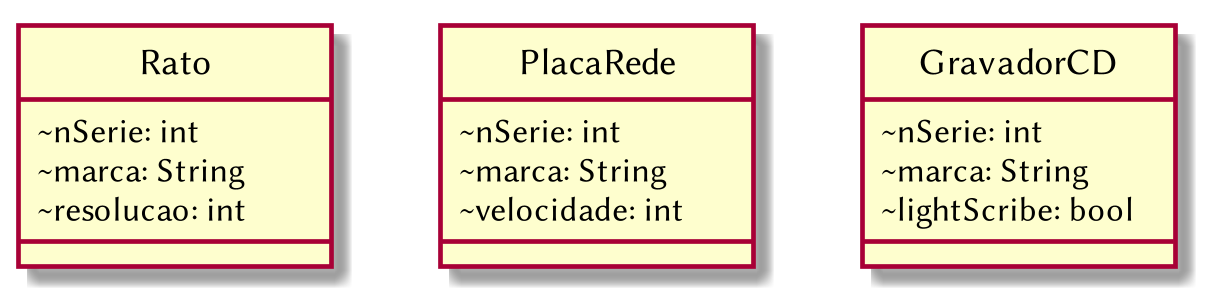
\includegraphics[width=0.5\linewidth]{./uml_diagrams/class7}
\end{center}
\end{frame}

\begin{frame}{Solução}
\begin{columns}
\column[]{0.5\linewidth}
\begin{center}
    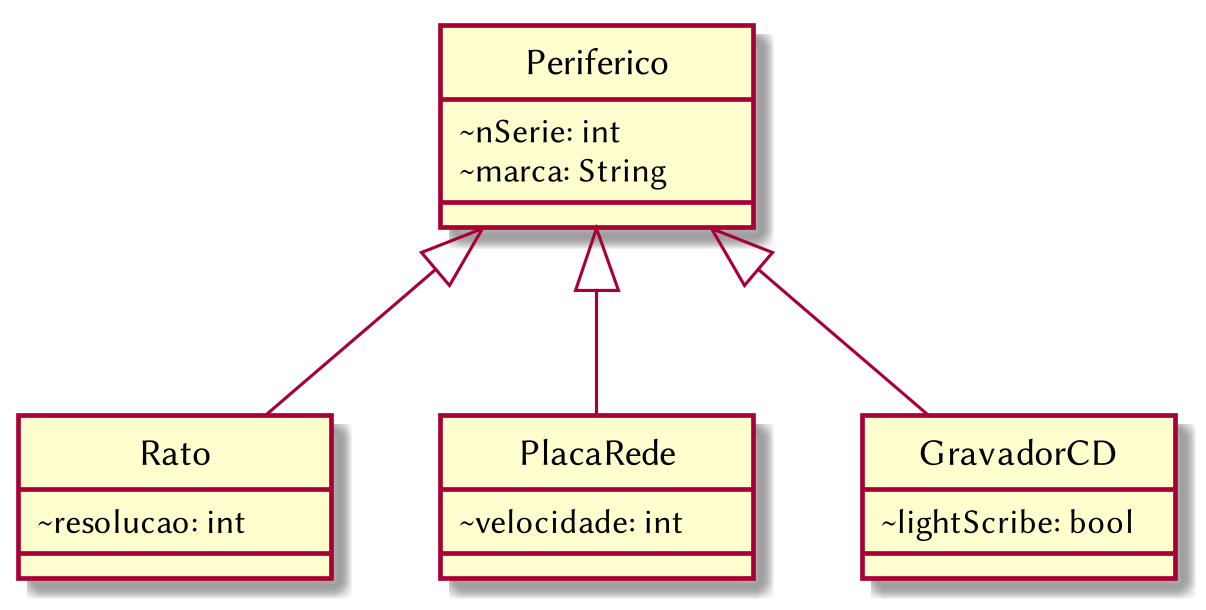
\includegraphics[width=\linewidth]{./uml_diagrams/class8}
\end{center}
\column[]{0.5\linewidth}
\begin{itemize}
    \item A seta lê-se \textit{is a}
    \item Rato \textit{is a} Periférico, etc.
    \item A direção da seta é importante, ou seja, não podemos dizer ``Periferico \textit{is a} Rato''
    \item Se ao lermos o diagrama a relação \textit{is a} não fizer sentido,  cuidado!
    \item Periférico é um tipo mais geral
    \item Rato é um tipo especializado de Periférico
    \item As subclasses herdam os membros da superclasse
    \item Os objetos da subclasse sabem responder às mensagens definidas na superclasse, porque \textit{is a}
\end{itemize}
\end{columns}
\end{frame}


\begin{frame}[fragile]{UML \textit{vs.}\ Java}
\begin{columns}
\column[]{0.5\linewidth}
\begin{center}
    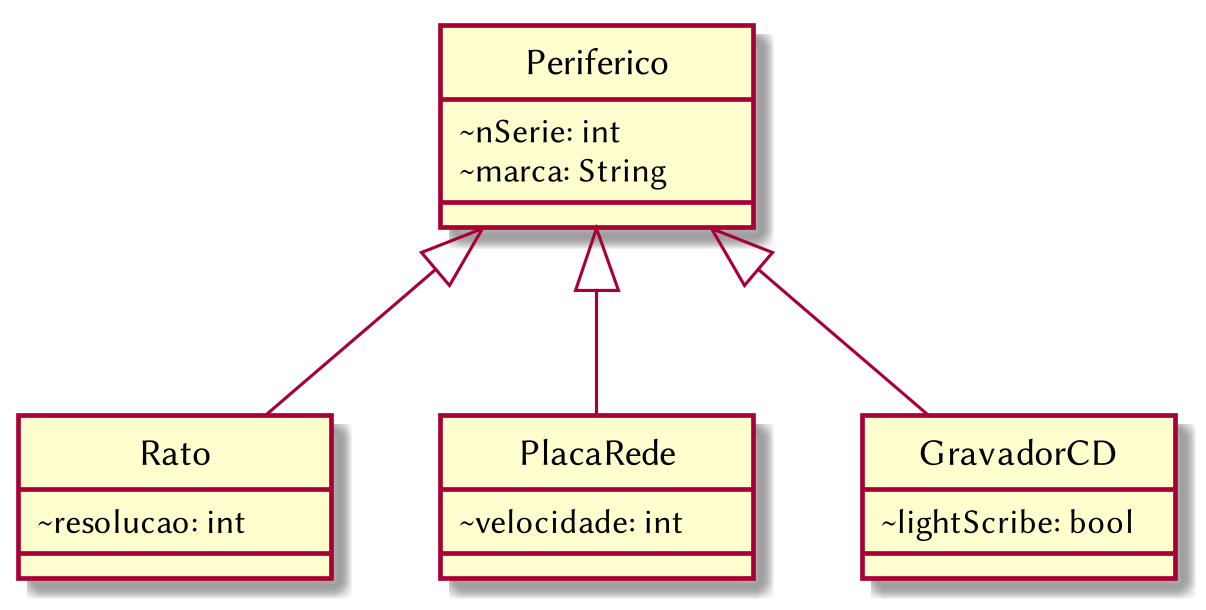
\includegraphics[width=\linewidth]{./uml_diagrams/class8}
\end{center}
\column[]{0.5\linewidth}
\scriptsize
\begin{minted}{java}
    class Periferico {
        int nSerie;
        String marca;
    }
    
    class Rato extends Periferico {
        int resolucao;
    }
    
    class PlacaRede extends Periferico {
        int velocidade;
    }
    
    class GravadorCD extends Periferico {
        boolean lightScribe;
    }
\end{minted}
\end{columns}
\end{frame}

\begin{frame}[fragile]{Instanciar subclasse}
\begin{columns}
    \column[]{0.5\linewidth}
    \begin{center}
        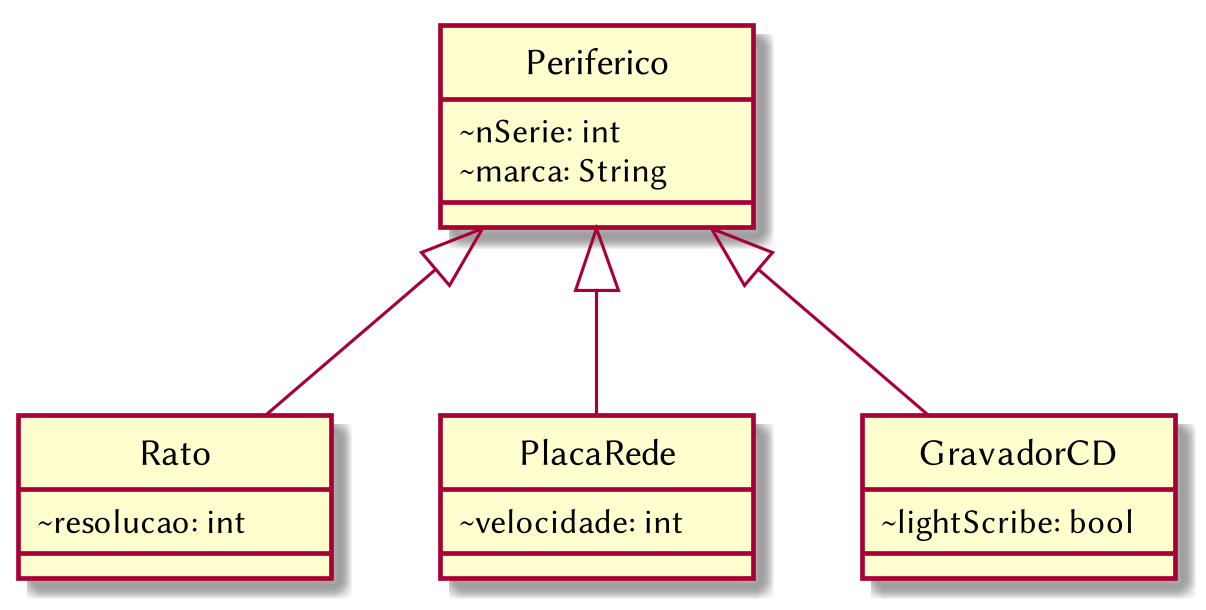
\includegraphics[width=\linewidth]{./uml_diagrams/class8}
    \end{center}
    \column[]{0.5\linewidth}
    \begin{minted}{java}
    Rato jerry = new Rato();
    \end{minted}
\begin{itemize}
    \item Podemos imaginar um objeto em memória com o seguinte aspeto:
    \begin{center}
        \begin{tabular}{|c|}
            \hline\\
            \textbf{:Periferico}\\
            \hline\\
            nSerie = 0\\
            marca = null\\
            \hline
            \hdashline\\
            \hline
            jerry : \textbf{Rato}\\
            \hline\\
            resolucao = 0\\
            \hline
        \end{tabular}
    \end{center}
\end{itemize}
\end{columns}
\end{frame}

\begin{frame}{Instanciar subclasse $\ldots$}
\begin{itemize}
    \item Notas importantes:
    \begin{itemize}
        \item Quando instanciamos uma subclasse, se a superclasse:
        \begin{itemize}
            \item não tiver um construtor definido, a JVM chama o construtor vazio da superclasse automaticamente
            \item tiver construtor definido, é da responsabilidade da subclasse chamar o construtor da superclasse 
        \end{itemize}
    \item A chamada ao construtor da superclasse é feita:
    \begin{itemize}
        \item  no construtor da subclasse, e é a primeira coisa a fazer antes de qualquer outra coisa
        \item através de \mintinline{java}{super()}, i.e., \mintinline{java}{super()} refere-se ao construtor da superclasse e, poderá ter, ou não, argumentos (i.e., depende do construtor da superclasse)
    \end{itemize}
    \end{itemize}
\end{itemize}
\end{frame}


\begin{frame}[fragile]{Exemplo}
    \begin{columns}  
        \column[]{0.4\linewidth}
        \scriptsize
\begin{minted}{java}
    class Periferico {
        int nSerie;
        String marca;
        
        Periferico(int n, String m) {
            nSerie = n;
            marca = m;
        }
    
        int getSerie() {
            return nSerie;
        }
    
        void setSerie(int n) {
            nSerie = n;
        }
    }
\end{minted}
\column[]{0.6\linewidth}
        \scriptsize
\begin{minted}{java}   
    class Rato extends Periferico {
        int resolucao;
        
        Rato() {
            super(0, "Nada");
            resolucao = 0;
        }
        
        Rato(int n, String s, int res) {
            super(n, s);
            resolucao = res;
        }
    }
    \end{minted}
\begin{itemize}
    \item No \mintinline{java}{main}:
\begin{minted}{java}
Rato r1 = new Rato();
Rato r2 = new Rato(123, "Logitech", 300);
System.out.print(r1.getSerie());  // 0
System.out.print(r2.getSerie());  // 123
\end{minted}
\end{itemize}
\end{columns}
\end{frame}


\begin{frame}{Class abstrata}
\begin{itemize}
    \item Uma classe que tem zero ou mais métodos sem implementação (i.e., abstratos)
    \item Uma classe abstrata tem de ser declarada como \mintinline{java}{absract}, assim como todos os métodos sem corpo
    \item Quem herda dessa classe é obrigado a implementar os métodos abstratos, ou também tem de ser declarada como abstrata
    \item Uma classe abstrata não pode ser instanciada
    
    \item Uma classe abstrata sem métodos abstratos apenas restringe a instanciação dessa classe
\end{itemize}
\end{frame}

\begin{frame}[fragile]{Exemplo}
\begin{columns}  
\column[]{0.4\linewidth}
\scriptsize
\begin{minted}{java}
    abstract class Periferico {
        int nSerie;
        String marca;
        
        Periferico(int n, String m) {
            nSerie = n;
            marca = m;
        }
        
        int getSerie() {
            return nSerie;
        }
        
        void setSerie(int n) {
            nSerie = n;
        }
    
        abstract void imprimir();
    }
\end{minted}
\column[]{0.6\linewidth}
\scriptsize
\begin{minted}{java}   
class Rato extends Periferico {
    int resolucao;
    
    Rato(int n, String s, int res) {
        super(n, s);
        resolucao = res;
    }
    
    void imprimir() {
        System.out.println("Isto é um rato");
        System.out.println("Marca: " + marca);
        System.out.println("Resolução:" + resolucao);
    }
        
}
\end{minted}
\begin{itemize}
\item No \mintinline{java}{main}:
\begin{minted}{java}
Rato r2 = new Rato(123, "Logitech", 300);
r2.imprimir();
\end{minted}
\end{itemize}
\end{columns}
\end{frame}


\begin{frame}[fragile]{Coleções (e.g., \mintinline{java}{ArrayList, LinkedList}) de instâncias de subclasses}
\begin{columns}
\column[]{1\linewidth}
\begin{itemize}
    \item \texttt{Rato, PlacaRede, GavadorCD} são todas subclasses de \texttt{Periferico}
    \item Por outras palavras, \texttt{Rato, PlacaRede, GavadorCD} \textit{is a} \texttt{Periferico}
    \item Assim, instâncias destas podem ``viver'' numa coleção do tipo da superclasse:
\begin{minted}{java}
    Rato r = new Rato();
    PlacaRede p = new PlacaRede();
    List<Periferico> al = new ArrayList<>();
    al.add(r);
    al.add(p);
    al.add(new GravadorCD());
\end{minted}
\item O que permite fazer:
\begin{minted}{java}
    for (Periferico p : al):
        p.imprimir();
\end{minted}
\end{itemize}
\column[]{0\linewidth}
\end{columns}
\end{frame}

\begin{frame}[fragile]{\mintinline{java}{instanceof}}
\begin{itemize}
    \item Permite ``perguntar'' ao objeto qual a classe da qual foi instanciado
\end{itemize}
\begin{columns}
\column[t]{0.5\linewidth}
\scriptsize
\begin{minted}{java}
Rato r = new Rato();
PlacaRede p = new PlacaRede();
List<Periferico> al = new ArrayList<>();
al.add(r);  // cast implícito de Rato p/Periférico
al.add(p);  // idem de PlacaRede
al.add(new GravadorCD());  // idem de GravadorCD

Periferico g = new GravadorCD();  // idem
\end{minted}
\column[t]{0.5\linewidth}
\scriptsize
\begin{minted}{java}
    for (Periferico p : al) {
        if (p instanceof Rato)
            System.out.println("É um rato");
        else if (p instanceof GravadorCD)
            System.out.println("É um gravador");
        else
            System.out.println("É o outro");
    }

    if (g instanceof GravadorCD)
        System.out.println("É um gravador");
\end{minted}
\end{columns}
\end{frame}

\begin{frame}[fragile]{Upcast \textit{vs.}\ Downcast}
\begin{itemize}
    \item \textbf{Upcast}
    \begin{itemize}
        \item conversão de um objeto de uma subclasse para o tipo da superclasse
        \item pode ser feito implicitamente ou explicitamente
\begin{minted}{java}
    Periferico g = new GravadorCD();  // upcast implícito
    Periferico h = (Periferico)new GravadorCD();  // upcast explícito
\end{minted}
    \end{itemize}
    \item \textbf{Downcast}
    \begin{itemize}
        \item conversão de um objeto de uma superclasse para o tipo de uma das subclasses 
        \item apenas pode ser feito explicitamente
\begin{minted}{java}
    Periferico p = new GravadorCD();  // upcast implícito
    GravadorCD i = p;  // downcast implícito ERRO (Incompatible types)
    GravadorCD h = (GravadorCD)p;  // downcast explícito OK
    Rato r = (Rato)p;  // downcast explícito aceite, mas...
\end{minted}
\item O último caso é aceite pela JVM durante a compilação, mas vamos ter uma \mintinline{java}{ClassCastException} em runtime
    \end{itemize}
\end{itemize}
\end{frame}

\end{document}


